\documentclass[../analysisII_notes.tex]{subfiles}
\begin{document}
\section{Aula 09 - 02 de Abril, 2025}
\subsection{Motivações}
\begin{itemize}
	\item Outras Classes de Integração.
\end{itemize}
\subsection{Outras Classes de Integração.}
\begin{prop*}
	Se f e g são funções Riemann-integráveis no intervalo \([a, b]\), então:
	\begin{itemize}
		\item[a)] O produto delas também é Riemann-integrável:
		      \[
			      f \cdot g\in \mathcal{R}([a, b]);
		      \]
		\item[b)] O módulo delas também será Riemann-integrável: definindo \(|f|:[a, b]\rightarrow \mathbb{R}\) como \(|f|(x)=|f(x)|\) para todos os pontos no domínio da função f, então \(|f|\) é integrável; além disso,
		      \[
			      \biggl\vert \int_{a}^{b}f(x)dx \biggr\vert\leq \int_{a}^{b}|f(x)|dx.
		      \]
		      Em particular, se \(|f(x)|\leq K\) para todo x no domínio - ou seja, se f for limitada em módulo - então
		      \[
			      \biggl\vert \int_{a}^{b}f(x)dx \biggr\vert\leq K(b-a).
		      \]
		\item[c)] Se g é uma função que nunca assume o valor 0 e tem módulo limitado inferiormente por \(\alpha \) (\(|g(x)|\geq \alpha > 0\)) para os pontos em \([a, b]\), então o quociente de f por ela também é integrável:
		      \[
			      g(x)\neq 0 \: \forall x\in [a, b] \Rightarrow \frac{f}{g}\in \mathcal{R}([a, b]).
		      \]
	\end{itemize}
\end{prop*}
\begin{figure}[H]
	\begin{center}
		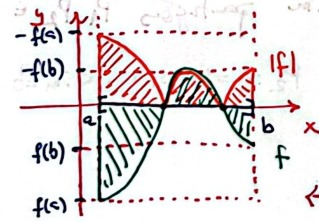
\includegraphics[height=0.5\textheight, width=0.5\textwidth, keepaspectratio]{./Images/unbound_modulus_08.png}
	\end{center}
	\caption{a f possui ``áreas negativas'' abaixo do seu gráfico.}
	\label{unbmod08}
\end{figure}
\begin{figure}[H]
	\begin{center}
		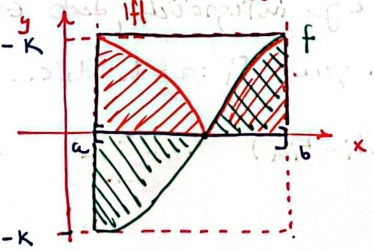
\includegraphics[height=0.5\textheight, width=0.5\textwidth, keepaspectratio]{./Images/bound_modulus_08.png}
	\end{center}
	\caption{por outro lado, quando o módulo é limitado por um número K, a área do retângulo de base b-a e altura K é um valor o qual a área sob o gráfico da \(|f|\) não pode superar.}
	\label{bddmod08}
\end{figure}
\begin{proof*}
	(i) Dada uma partição
	\[
		\mathcal{P}: a = t_{0} < t_{1} < \dotsc < t_{n} = b,
	\]
	denote, para cada i entre 1 e n,
	\begin{align*}
		 & \omega_{i}(f)\coloneqq \sup_{}\{|f(x)-f(y)|:\:x, y\in [t_{i-1}, t_{i}]\}         \\
		 & \omega_{i}(f)\coloneqq \sup_{}\{|g(x)-g(y)|:\:x, y\in [t_{i-1}, t_{i}]\}         \\
		 & \omega_{i}(fg)\coloneqq \sup_{}\{|(fg)(x)-(fg)(y)|:\:x, y\in [t_{i-1}, t_{i}]\},
	\end{align*}
	as respectivas oscilações de f, g e \(fg\) no i-ésimo subintervalo de \(\mathcal{P}\). Para todos os pontos x, y do intervalo \([a, b]\), temos
	\begin{align*}
		|(fg)(x)-(fg)(y)| & = |f(x)g(x)-f(x)g(y)+f(x)g(y)-f(y)g(y)|        \\
		                  & \leq |f(x)||g(x)-g(y)|+|f(x)-f(y)|\cdot |g(y)| \\
		                  & \leq K|g(x)-g(y)| + K |f(x)-f(y)|,
	\end{align*}
	em que o número K é positivo e escolhido como um número limitando tanto o módulo de f, quanto o de g (note que sua existência é garantida pelo fato de ambas serem limitadas em módulo, aí basta pegar K como o máximo dos limitadores delas). Assim, concluímos que, para todo \(i=1,2,\dotsc ,n\),
	\[
		\omega_{i}(fg)\leq K(\omega_{i}(f)+\omega_{i}(g)).
	\]
	Logo,
	\[
		L(fg; \mathcal{P})\leq K [(U(f; \mathcal{P})-L(f; \mathcal{P})) + (U(g; \mathcal{P})-L(g; \mathcal{P}))]
	\]
	e, sendo ambas integráveis, para cada \(\varepsilon >0\), existem partições \(\mathcal{P}_{1}, \mathcal{P}_{2}\) do intervalo \([a, b]\), dadas por
	\begin{align*}
		 & \mathcal{P}_{1}: a=t_{0}<t_{1}<\dotsc <t_{n}=b   \\
		 & \mathcal{P}_{2}: a = s_{0}<s_{1}<\dotsc <s_{m}=b
	\end{align*}
	tais que
	\begin{align*}
		 & \sum\limits_{i=1}^{n}\omega_{i}(f)(t_{i}-t_{i-1})<\frac{\varepsilon }{2K}  \\
		 & \sum\limits_{j=1}^{m}\omega_{j}(g)(s_{j}-s_{j-1})<\frac{\varepsilon }{2K}.
	\end{align*}
	Sendo assim, colocamos \(\mathcal{P}\) como a partição dada pela união das duas \(\mathcal{P}_{1}\) e \(\mathcal{P}_{2}\), donde concluímos que
	\begin{align*}
		U(fg; \mathcal{P}) & \leq K[(U(f; \mathcal{P})-L(f; \mathcal{P})) + (U(g; \mathcal{P})-L(g; \mathcal{P}))]                 \\
		                   & \leq K[(U(f; \mathcal{P}_{1})-L(f; \mathcal{P}_{1})) + (U(g; \mathcal{P}_{2})-L(g; \mathcal{P}_{2}))] \\
		                   & < K \biggl[\frac{\varepsilon }{2K}+\frac{\varepsilon }{2K}\biggr]=\varepsilon,
	\end{align*}
	concluindo que fg é integrável.

	Com respeito ao segundo, lembre-se que para quaisquer elementos x, y no intervalo em que a f está definida, temos a continuidade do módulo como função:
	\[
		\biggl\vert |f(x)|-|f(y)| \biggr\vert \leq |f(x) - f(y)|.
	\]
	Dessa forma, dado um \(\varepsilon \) positivo, escolha uma partição \(\mathcal{P}_{0}\) do intervalo \([a, b]\), tal que
	\[
		\sum\limits_{i=1}^{n}\omega_{i}(f)(t_{i}-t_{i-1})<\varepsilon,
	\]
	a qual existe pois supomos que f é integrável. Além disso, note que, para todos os elementos nos pontos das partições, o módulo impede que a oscilação ``atinja'' os valores negativos da função - é como se a altura da função em módulo fosse menor do que ela sem nada. Assim,
	\[
		\omega_{i}(|f|)\leq \omega_{i}(f) \Rightarrow \sum\limits_{i=1}^{n}\omega_{i}(|f|)(t_{i}-t_{i-1}) \leq \sum\limits_{i=1}^{n}\omega_{i}(f)(t_{i}-t_{i-1}) < \varepsilon.
	\]
	Portanto, pelo \hyperlink{integrability_conditions}{\textit{critério de Riemann}}, o módulo de f é integrável em \([a, b]\). \qedsymbol

	O item (iii) ficará de exercício.
\end{proof*}
\begin{example}
	A recíproca não vale, ou seja, se o módulo de uma função for integrável dentro do intervalo \([a, b]\), a função sem o módulo não necessariamente será. Para ver isso, basta considerar \(f:[0, 1]\rightarrow \mathbb{R}\) dada por
	\[
		f(x) = \left\{\begin{array}{ll}
			1,  & \quad x\in \mathbb{Q}\cap [0, 1]     \\
			-1, & \quad x\not\in \mathbb{Q}\cap [0,1].
		\end{array}\right.
	\]
	Vemos que \(|f|\) é identicamente igual à 1 em \([0, 1]\), o que torna-a uma função constante, a qual é integrável. Porém,
	\[
		\underline{\intup_{0}^{1}}f = -1 \quad\&\quad \overline{\intup_{0}^{1}}f = 1.
	\]
	\begin{exr}
		Verifique os valores das integrais acima.
	\end{exr}
\end{example}
\subsection{Considerações Finais: o que ficou de fora.}
Nessas considerações finais, queremos provar algumas coisas que ficaram faltando.
\begin{theorem*}
	Sejam \(f, g :[a, b]\rightarrow \mathbb{R}\) funções limitadas tais que:
	\begin{itemize}
		\item[i)]As funções coincidem para todos os pontos de \([a, b]\), a menos de um conjunto finito deles:
		      \[
			      g(x)=f(x) \forall x\in [a, b]\setminus{D},\quad D\subsetneq [a, b] \;\&\; |D|<\infty;
		      \]
		\item[ii)] f é Riemann-integrável e sua integral coincide com g:
		      \[
			      \int_{a}^{b}g = \int_{a}^{b} f.
		      \]
	\end{itemize}
	Então, g também é Riemann-integrável.
\end{theorem*}
\begin{proof*}
	Com efeito, seja
	\[
		D = \{x_{1}<x_{2}<\dotsc <x_{n}\}\subseteq [a, b]
	\]
	o conjunto dos pontos tais que \(f(x)\) difere de \(g(x)\) e defina \(h:[a, b]\rightarrow \mathbb{R}\) dada por
	\[
		h(x)\coloneqq g(x)-f(x) \; \forall x\in [a, b].
	\]
	Observe, então, que
	\[
		h(x) = 0,\; \forall x\in [a, b]\setminus{D}
	\]
	e que
	\[
		h(x)\neq 0,\; \forall x\in D.
	\]

	\begin{figure}[H]
		\begin{center}
			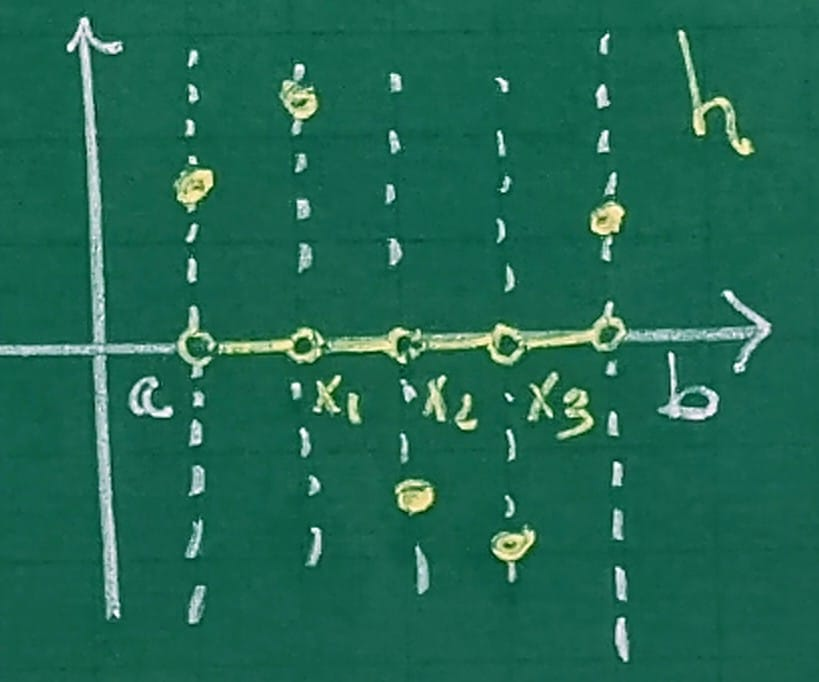
\includegraphics[height=0.5\textheight, width=0.5\textwidth, keepaspectratio]{./Images/stepfunc_09.png}
		\end{center}
		\caption{podemos pensar na h como um caso particular da função escada.}
		\label{stepfunc09}
	\end{figure}
	Com isso, definindo a partição
	\[
		\mathcal{P}_{0}: a = x_{0} \leq \underbrace{ x_1 < x_2 < \dotsc <x_{n}}_{D}\leq x_{n+1}=b,
	\]
	segue que, quando x está entre quaisquer pontos dessa partição,
	\[
		h(x) = 0 \quad \forall x\in (x_{i-1}, x_{i}),\; i = 1, 2, \dotsc , n+1,
	\]
	mostrando que h é uma função escada com \(c_{i}\) constantemente nula para todos os i's. Logo, ela é Riemann-integrável em \([a, b]\) com
	\[
		\int_{a}^{b}h = \sum\limits_{i=1}^{n+1}c_{i}(x_{i}-x_{i-1}) = 0.
	\]
	Finalmente, como \(g\) é, na verdade, a soma \(f + h\), o que provamos foi que
	\[
		\int_{a}^{b}g = \int_{a}^{b} f + \int_{a}^{b} h = \int_{a}^{b} f.\quad \text{\qedsymbol}
	\]
\end{proof*}
Anteriormente, provamos o \hyperlink{integral_additivity}{\textit{teorema da aditividade das componentes da integral}}, mas acabamos por deixar quieto a prova dele para as integrais em si. Sendo assim,
\begin{theorem*}[Aditividade da Integral]
	Se \(f:[a, b]\rightarrow \mathbb{R}\) é limitada, então f é integrável em \([a, b]\) se, e somente se, para todo número c entre a e b, as restrições da f aos cortes
	\[
		f|_{[a, c]} \quad\&\quad f|_{[c, b]}
	\]
	são ambas integráveis. Em caso afirmativo, tem-se
	\[
		\int_{a}^{b} f = \int_{a}^{c} f + \int_{c}^{b}f,\quad \forall a < c < b.
	\]
\end{theorem*}
\begin{proof*}
	\(\Rightarrow )\) Lembre-se que, pelo \hyperlink{integral_additivity}{\textit{teorema da aditividade das componentes da integral}}, temos
	\[
		\overline{\intup_{a}^{c}}f + \overline{\intup_{c}^{b}}f = \overline{\intup_{a}^{b}}f \geq \underline{\intup_{a}^{b}}f = \underline{\intup_{a}^{c}}f +\underline{\intup_{c}^{b}}f.
	\]
	Assim, se f é integrável, a desigualdade torna-se uma igualdade, tal que
	\[
		\overline{\intup_{a}^{c}}f + \overline{\intup_{c}^{b}}f = \overline{\intup_{a}^{b}}f = \underline{\intup_{a}^{b}}f = \underline{\intup_{a}^{c}}f +\underline{\intup_{c}^{b}}f.
	\]
	Logo,
	\[
		\overline{\intup_{a}^{c}}f + \overline{\intup_{c}^{b}}f = \underline{\intup_{a}^{c}}f +\underline{\intup_{c}^{b}}f
	\]
	e
	\[
		\int_{a}^{b} f = \int_{a}^{c} f + \int_{c}^{b} f.
	\]
	No entanto, ainda temos que mostrar a igualdade para cada parcela das somas. Para tal, temos
	\[
		0 = \biggl(\underbrace{\overline{\intup_{a}^{c}}f + \underline{\intup_{a}^{c}}f}_{\geq 0}\biggr) + \biggl(\underbrace{\overline{\intup_{c}^{b}}f + \underline{\intup_{c}^{b}} f}_{\geq 0}\biggr),
	\]
	donde ambas as parcelas devem ser nulas para que sua soma dê zero também. Consequentemente,
	\[
		\overline{\intup_{a}^{c}} f = \underline{\intup_{a}^{c}} f \quad\&\quad \overline{\intup_{c}^{b}}f = \underline{\intup_{c}^{b}}f.
	\]
	Portanto, as restrições são integráveis nos seus respectivos subintervalos.

	\(\Leftarrow )\) Reciprocamente, se as restrições são integráveis em seus respectivos subintervalos, o seguinte valerá para qualquer c entre a e b:
	\[
		{\color{red}\overline{\intup_{a}^{c}}f} + {\color{blue}\overline{\intup_{c}^{b}}f} = \overline{\intup_{a}^{b}}f =\underline{\intup_{a}^{b}}f = {\color{red}\underline{\intup_{a}^{c}}f} +{\color{blue} \underline{\intup_{c}^{b}}f}.
	\]
	Consequentemente, seguindo as cores,
	\[
		{\color{red}\underline{\intup_{a}^{c}}f} = {\color{red}\overline{\intup_{c}^{b}}f} \quad\&\quad {\color{blue}\overline{\intup_{c}^{b}}f} = {\color{blue}\underline{\intup_{c}^{b}}f}.
	\]
	Portanto,
	\[
		\int_{a}^{b}f = \int_{a}^{c} f + \int_{c}^{b}f.\quad \text{\qedsymbol}
	\]
\end{proof*}
\begin{tcolorbox}[
		skin=enhanced,
		title=Observação,
		fonttitle=\bfseries,
		colframe=black,
		colbacktitle=cyan!75!white,
		colback=cyan!15,
		colbacklower=black,
		coltitle=black,
		drop fuzzy shadow,
		%drop large lifted shadow
	]
	Se f é integrável em \([a, b]\), então
	\[
		\biggl\vert \int_{a}^{b}f \biggr\vert \leq \int_{a}^{b}|f|,
	\]
	pois, para todos os elementos do intervalo \([a, b]\),
	\[
		-|f(x)|\leq f(x)\leq |f(x)| \Rightarrow -\int_{a}^{b}|f|\leq \int_{a}^{b}f\leq \int_{a}^{b}|f|.
	\]
	Em particular, se \(|f(x)|\leq K\) para todo x em \([a, b]\), então
	\[
		\biggl\vert \int_{a}^{b}f \biggr\vert \leq \int_{a}^{b}|f|\leq \int_{a}^{b}K = K(b-a).
	\]
\end{tcolorbox}
\begin{theorem*}
	Seja \(f:[a, b]\rightarrow \mathbb{R}\) uma função limitada tal que, para todo c entre a e b, a restrição de f ao intervalo \([a, c]\) é integrável. Então, a f sem restrições é integrável e
	\[
		\int_{a}^{b}f = \lim_{c\to b^{-}}\int_{a}^{c}f.
	\]
	Vale o análogo para restrições em \([c, b]\).
\end{theorem*}
\begin{figure}[H]
	\begin{center}
		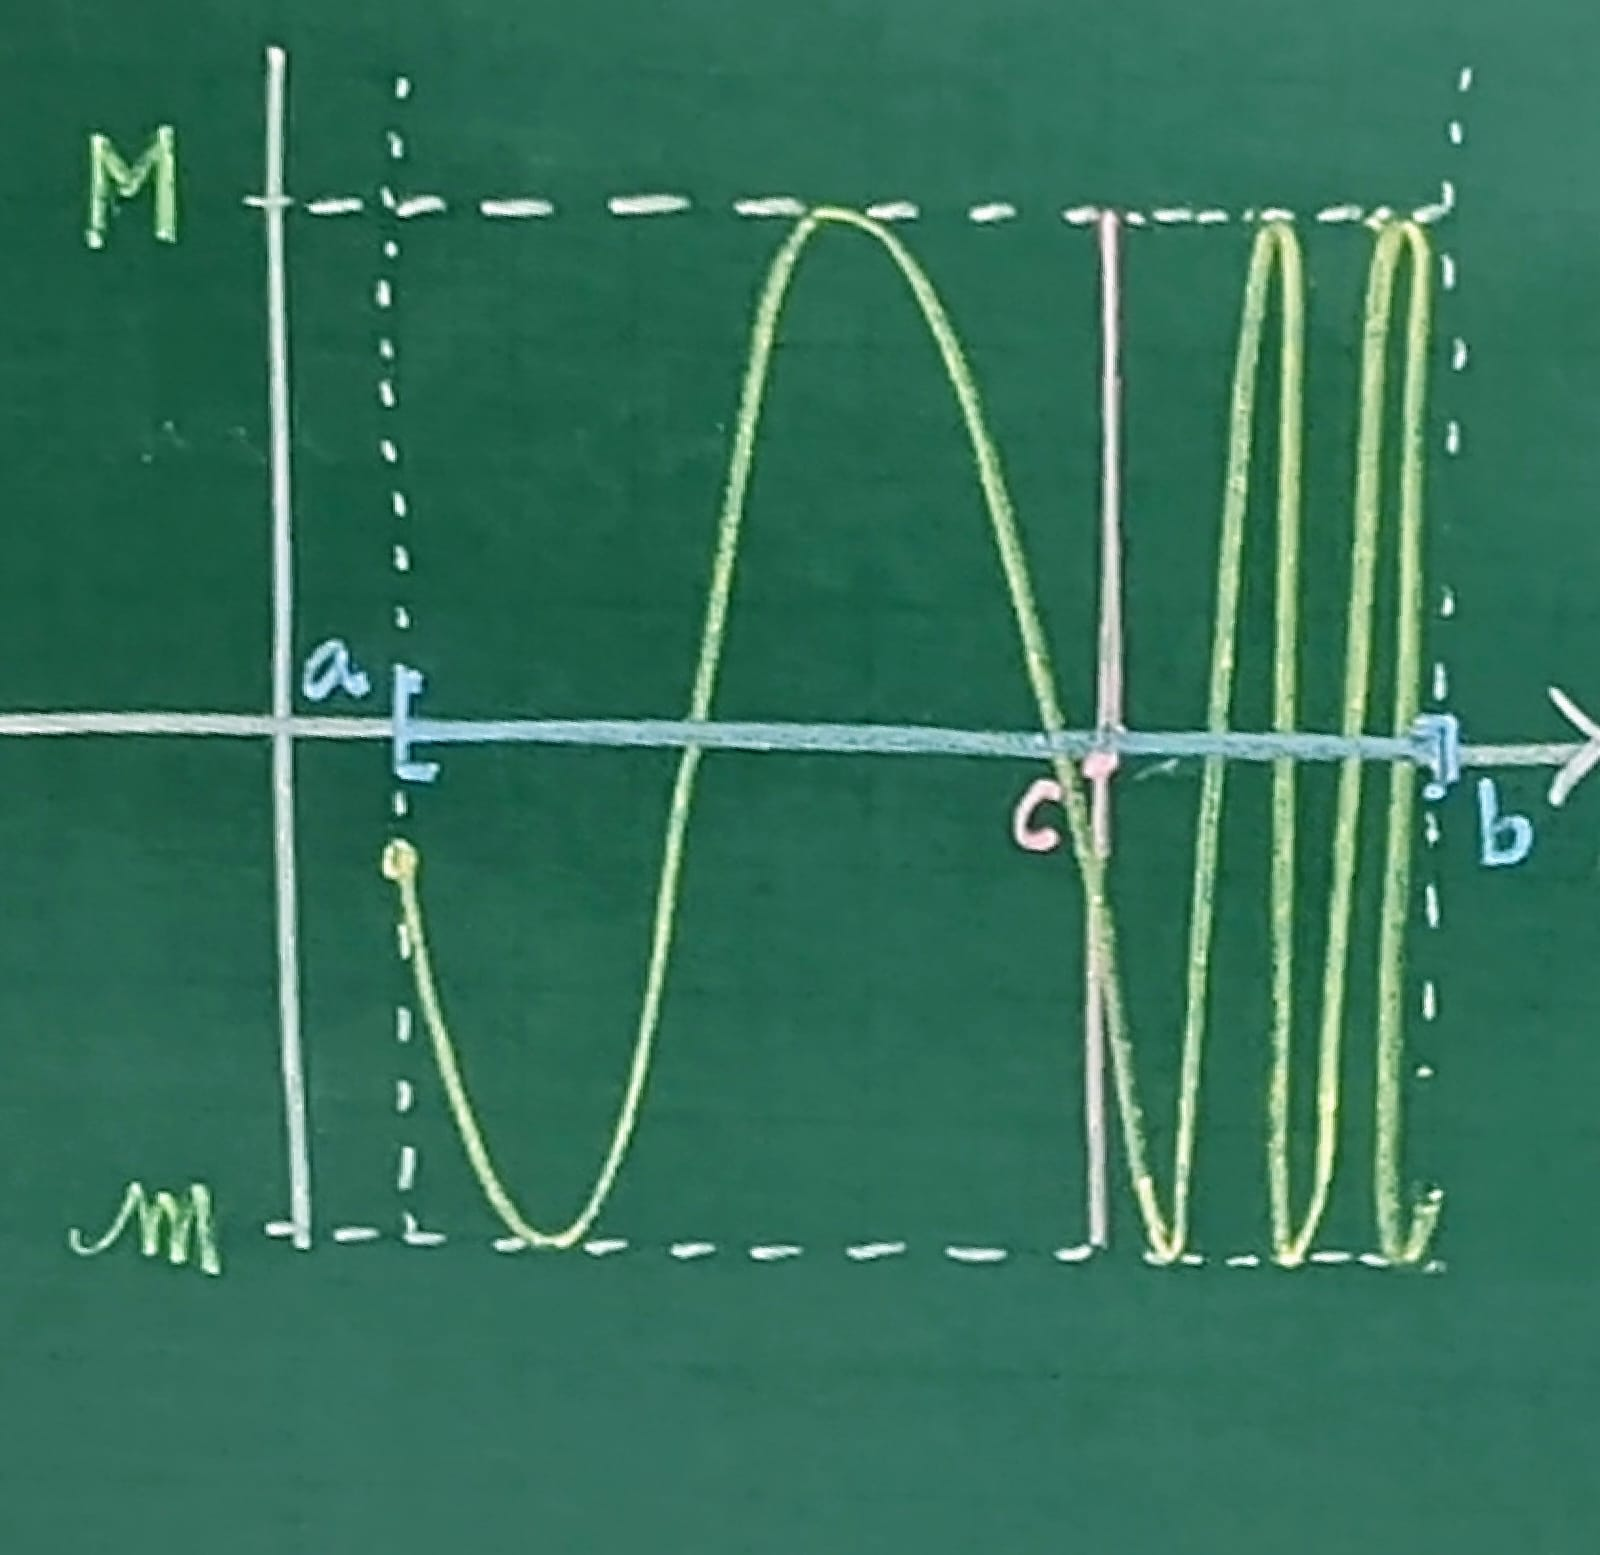
\includegraphics[height=0.5\textheight, width=0.5\textwidth, keepaspectratio]{./Images/squishy_09.png}
	\end{center}
	\caption{a função pode ter comportamento oscilatório ou patológico à esquerda, mas, pelas condições do teorema, a integral ainda pode existir.}
	\label{squish09}
\end{figure}
\begin{proof*}
	Primeiro, sejam
	\begin{align*}
		 & M \coloneqq \sup_{}f  \\
		 & m \coloneqq \inf_{}f,
	\end{align*}
	e podemos supor que \(m\) é menor que \(M\) (caso contrário, f seria constante e não teria o que fazer). Com base nisso, tomando \(\varepsilon \) positivo qualquer, escolha c entre a e b tal que
	\[
		b-c < \frac{\varepsilon }{2(M-m)}.
	\]
	Com esse c, sendo a restrição de f ao \([a, c]\) integrável, existe uma partição
	\[
		\mathcal{P}: a = t_{0} < t_{1} < \dotsc < t_{n} = c
	\]
	tal que, denotando por \(\omega_{i}\) a oscilação de f entre os pontos da partição:
	\[
		\omega_{i} = \sup_{\mathclap{x, y\in [t_{i-1}, t_{i}]}}|f(x)-f(y)|,
	\]
	então
	\[
		\sum\limits_{i=1}^{n}\omega_{i}(t_{i}-t_{i-1})<\frac{\varepsilon }{2}.
	\]
	Com isso, a oscilação na parte restante, \(\omega^{*}\), deve satisfazer
	\[
		\omega^{*}= \sup_{\mathclap{x, y\in [c, b]}}|f(x)-f(y)|\leq M-m.
	\]
	Logo, colocando
	\[
		\mathcal{P}_{0}: a = t_{0} < t_1 <\dotsc <t_{n} = c < t_{n+1} = b,
	\]
	teremos
	\[
		U(f; \mathcal{P}_{0}) - L(f; \mathcal{P}_{0}) = \sum\limits_{i=1}^{n}\omega_{i}(t_{i}-t_{i-1}) + \omega^{*}(b-c) < \frac{\varepsilon }{2} + (M-m)\frac{\varepsilon }{2(M-m)}.
	\]
	Portanto, a f é integrável. (O limite ficou para a próxima aula) \qedsymbol
\end{proof*}
\end{document}
